\chapter*[(First Warning to McDowell)]{Golgatha}

At this point, we are forced to start off with a theoretical digression---of the sort I have been trying my best to avoid. The deep, fundamental discrepancies between John's narrative on the one hand, and that of the Synoptic Evangelists on the other, are well-known (``How many gospels are there? Four? No: three and one'').\footnote{ Dmitry Merezhkovsky, \emph{Jesus the Unknown}, trans. H. Chrouschoff Matheson, p. 73. (Z.B.)} And Dmitry Merezhkovsky was probably right when he wrote that ``the dispute concerning John is the greatest enigma of Christianity... perhaps the enigma of Christ Himself.''\footnote{\emph{Jesus the Unknown}, p. 92.} To me, however---an irreligious person in general, and a complete virgin when it comes to theology---the coexistence of these two fundamentally irreducible and mutually irreconcilable versions seems perfectly normal and natural.

Strange as it may sound, it is actually my profession that has trained me to have such a perception. For us in the natural sciences, you see, knowledge is fundamentally reductive. Thus, as a rule, the continued coexistence of alternative conceptions of a natural phenomenon indicates that they are in fact complementary, and simply ``reduce'' observable reality to different aspects of its nature. As I see it, then, the opposition between John and the Synoptists is fundamentally no different from, say, the relationship between the wave and particle theories of light, which describe the same object in different ways, and only give an adequate impression of it when taken together as a pair. Again, let me quote from Merezhkovsky's apologia \emph{Jesus the Unknown} (pp. 97-98):

\begin{smallquote}
    John divines correctly---better perhaps than the synoptics---what Jesus \emph{intended}. What He \emph{did}, we learn from Mark; what He \emph{said}, from Matthew; what He \emph{felt}, from Luke. But what He \emph{intended}, we learn from John; and of course, it is what He intended that is of real, primary importance.\footnote{Emphasis Merezhkovsky's. (K.E.)}
\end{smallquote}

Now, that's all well and good on a general, conceptual level; in terms of the problem before us, though, where it is the specific details of the events that are important, the situation changes. We will frequently discover cases where John describes certain colorful incidents in detail that are completely absent from the Synoptists' narrative, and vice-versa---this is normal. In this sense, however, the scene at Golgotha is unique: here, the accounts of John and the Synoptists strike ``tit for tat,'' contradicting each other in literally every detail. And since my arguments are based on complete trust in the facts (though not necessarily their interpretations) reported by all four of the Evangelists, I find myself in a rather complex position, from which there is no clear way out.\footnote{However, one could still put forward the following hypothesis: the three Synoptic Gospels are genuine memoirs, whereas the Gospel of John was... let's say, a historical novel based on the others written many years later, in which truth and artistic license are melded into an inseparable whole. Furthermore, this second reality, owing to the genius (or Divine Inspiration, your choice) behind its creation, broke away, as one might expect, from its historical foundation and became entirely self-contained. I must admit that adopting such an assumption (which would allow me to disavow all of John's testimony) would make my life significantly easier. Alas! The starting conditions for the problem at hand (which include giving equal treatment to the four canonical texts) were defined quite strictly, and are not subject to review. (K.E.)}

% [htbp]: Instructs LaTeX to try placing the image Here, at the Top, Bottom, or on a separate Page (in that order).
\begin{figure}[htbp]
    \centering
    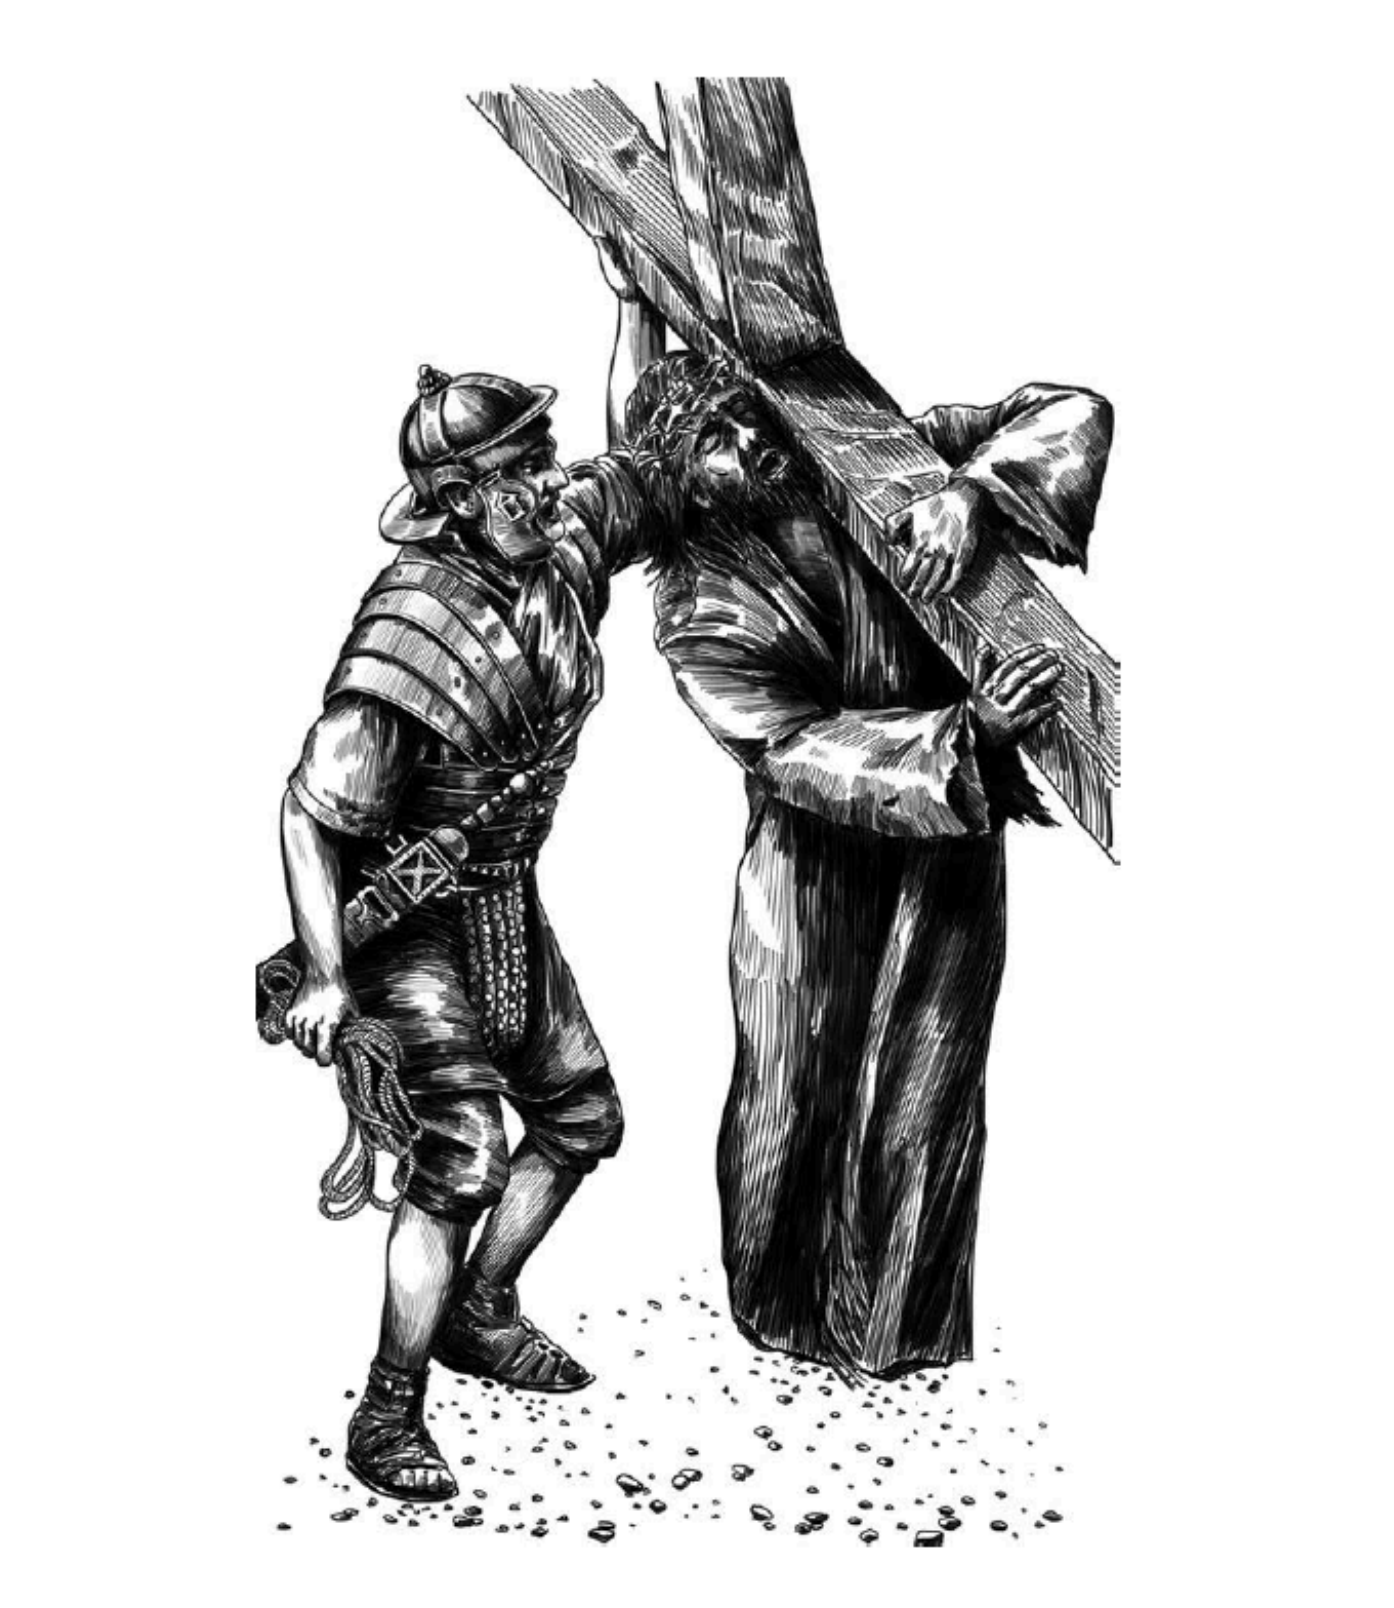
\includegraphics[width=1\textwidth]{assets/golgatha.png}
    \label{fig:golgatha}
\end{figure}

The discrepancies begin with a typical ``trifle.'' John confidently testifies that Jesus, ``bearing His cross, went out to a place called the Place of a Skull, which is called in Hebrew, Golgotha'' (Jn 19:17). Meanwhile, the Synoptists unanimously claim that the Savior's cross was carried by a certain Simon of Cyrene, and even include completely verifiable biographical details about the man, calling him ``the father of Alexander and Rufus'' (Mt 27:32, Mk 15:21, Lk 23:26). This time, you can't take lofty refuge in the nature of the Logos at hand, and you can't get out of this one with a casuistry like ``both of them are right, but each in their own way.'' You have to answer honestly: who got mixed up here?

I once heard the following, purely philological argument in support of the Gospels' authenticity as historical documents. It concerns a widely known episode:

\begin{smallquote}
    And about the ninth hour Jesus cried out with a loud voice, saying, ``Eli, Eli, lama sabachthani?'' that is, ``My God, My God, why have You forsaken Me?'' Some of those who stood there, when they heard that, said, ``This Man is calling for Elijah!'' Immediately one of them ran and took a sponge, filled it with sour wine and put it on a reed, and offered it to Him to drink. The rest said, ``Let Him alone; let us see if Elijah will come to save Him.'' (Mt 27:46-49)
\end{smallquote}

So (if I understand correctly), the use of unannotated direct speech to reveal the motivations of side characters only emerged as a literary device with the advent of the European psychological novel, in the 19\textsuperscript{th} century; therefore, what we are dealing with is the stenographically accurate record of an eyewitness. Perhaps this is because I am not a philologist, but this sounds completely convincing to me. However, I should point out that the argument refers specifically to the Synoptists' narrative---dry as a report, and therefore especially sorrowful. It is in their account that a Man dies betrayed and abandoned by all those around him---a far cry from the figures of chromium-molybdenum steel who feature in \emph{Lives of the Saints}.

In the Gospel of John, of course, these words are nowhere to be found. On the other hand, you find, for example, a quotation from Jewish scripture that Roman soldiers casually recite verbatim (Jn 19:24)---just in case the people around them fail to notice that they are not merely casting lots for a dead man's clothes, but fulfilling an ancient prophecy? There is also the sublime conversation that a dying man, suffering the most terrible of agonies, carries on with the people standing at his cross: his mother and the ``disciple whom he loved,'' that is, John (Jn
19:26-27).\footnote{McDowell provides a detailed description of the medical aspects of crucifixion. It is often believed that death results from shock, combined with dehydration and heatstroke, but that is actually somewhat inaccurate. Several hours after crucifixion, a person starts to develop pulmonary edema due to the difficulty in breathing; the immediate cause of death is asphyxiation. Hence, a person undergoing crucifixion is incapable of holding an extended, coherent conversation as a matter of principle. (K.E.)}

Wait a second! Among other things, the Synoptists have neither his mother nor his disciple there at all. The only ones there are the Galilean women who follow Christ everywhere---Mary Magdalene, Mary, mother of James, and Salome---and they are not standing anywhere near the cross, but are looking on \emph{from a distance} (Mk 15:40, Mt 27:55). How could it be that all three Synoptists failed to notice such a ``small detail'' as John and the Virgin Mary \emph{standing at the cross}? Especially since Ivan Bezdomny's vision of Bald Mountain quite inaptly springs to mind: ``and the mountain was encircled by a double cordon.''\footnote{\emph{The Master and Margarita}, p. 143.} Of course, you could hardly call that authoritative---and yet... I honestly admit that I have no idea what to do here---unless I adopt Merezhkovsky's interpretation and come to the straightforward, yet depressing conclusion that the Savior merely \emph{wanted} his mother and his beloved disciple at his cross...

Where am I going with this? Well, taking on the role of counterintelligence agent Philip Rawlings, who ``doesn't believe anything he hears, and very little of what he sees,''\footnote{Ernest Hemingway, \emph{The Fifth Column and Four Stories of the Spanish Civil War}, p. 27} I just can't help but wonder: was the man who was crucified between two robbers at noon on the fourteenth day of the spring month of Nisan\footnote{This specific phrasing for the date of Jesus' death is used several times throughout \emph{The Master and Margarita} (e.g. p. 13, p. 255). (Z.B.)} really the same man who, six days before, had entered Jerusalem to the cheers of ``Hosanna''? If the conversation with his mother and disciple really took place the way John reported it, then yes, absolutely. But if nothing took place on Golgotha other than what the Synoptists so meticulously described, then I'm sorry, but just about anybody could have been hanging on the middle cross---perhaps a robber just like the two others, or perhaps a Zealot partisan.

One need only assume that, for their own benefit, the Roman authorities wanted to strengthen the position of Jesus' sect, and that he made a deal with them (``the end justifies the means'')---and there would be practically nothing left unclear in the entire story of the Resurrection. This, incidentally, would explain the role of the episode where Jesus is dressed in a scarlet military cloak---after his trial, but before his scourging and his ascent of Golgotha (for example, Mk 15:17-20). After the scourging, they put Jesus' clothes on another man---the man who was to take his place on the middle cross.

Personally, I don't intend on defending this theory, or even seriously analyzing it, as that would force me to reject the ``presumption of honesty'' that I am obliged to uphold (in accordance with the starting conditions). But while I have the right to make such a ``withdrawal,'' McDowell does not. And considering that he took the time to craft a completely serious argument against the \emph{Passover Plot} hypothesis, where not a single fact adds up, and Christ and Joseph of Arimathea cheat side-by-side like a pair of train station cardsharps, he is simply obliged to examine a hypothesis as patently obvious as the ``Uncrucified Christ.''

At the same time, however, by no means do I wish to say that McDowell's position on that issue would be indefensible. He could most likely cite the high priests who visited the execution site (Mt 27:41) or the conversation with the remorseful robber: ``Assuredly, I say to you, today you will be with Me in Paradise'' (Lk 23:43). In turn, an ardent supporter of this hypothesis could object that the face of the man on the cross was disfigured beyond all recognition in any case; that the high priests certainly did not come up close to the cross, and a person undergoing crucifixion (assuming it takes place not in a classical painting, but in real life) is forced to keep their face lowered to the ground; that the organizers of the hoax surely would have taken care to increase the physical resemblance of the people involved; that the conversation with the robber could not have been heard by anyone apart from the legionnaires, and their ``testimony'' is clearly worthless, etc. In short, both sides would have wide room to maneuver here.

However, the problem lies not in these particularities. Even if McDowell manages to provide a sufficiently convincing rebuttal of the ``Uncrucified Christ'' hypothesis, his position will not become any less unenviable. After all, his entire \emph{system} of proof is based on the assumption that he has analyzed (and refuted) \emph{every} possible materialist theory---and suddenly, a special case pops up... It just goes to show that the range of logical possibilities is fundamentally inexhaustible, and there's nothing you can do about it.

In short, it seems that McDowell's dreadnought has already struck a sea mine on its way out of the harbor. And while the crew's efforts might keep the ship afloat, its use as a combat unit will be rather limited from here on out. However, there are even greater surprises in store for Captain McDowell on this voyage...